\section{Drift Chambers (DC)}

\subsection{Geometry}

The DC geometry is implemented through the COATJAVA geometry service.
The service provides the Geant4 definitions that are read by the GEMC perl API to build the geometry database.

For each sector, there are three drift chambers: one in front of the torus, one between the torus coils
and one following the torus.  These three chambers are referred to as different ``regions''.
The chambers are strung with the wires arranged in 12 internal layers.
Each layer is a generic G4Trapezoid, tilted by $+6^O$ or $-6^O$ depending if they are in the first or second
superlayer of a region.
The 12 layers in each region (6 per superlayer) are placed in a region mother volume made of air, see \F{dcGeometry}.
The layers are assigned the $CO_2$ material and associated with the DC hit process routine.
The wire identification is performed in the Process ID routine.

\begin{figure}
	\centering
	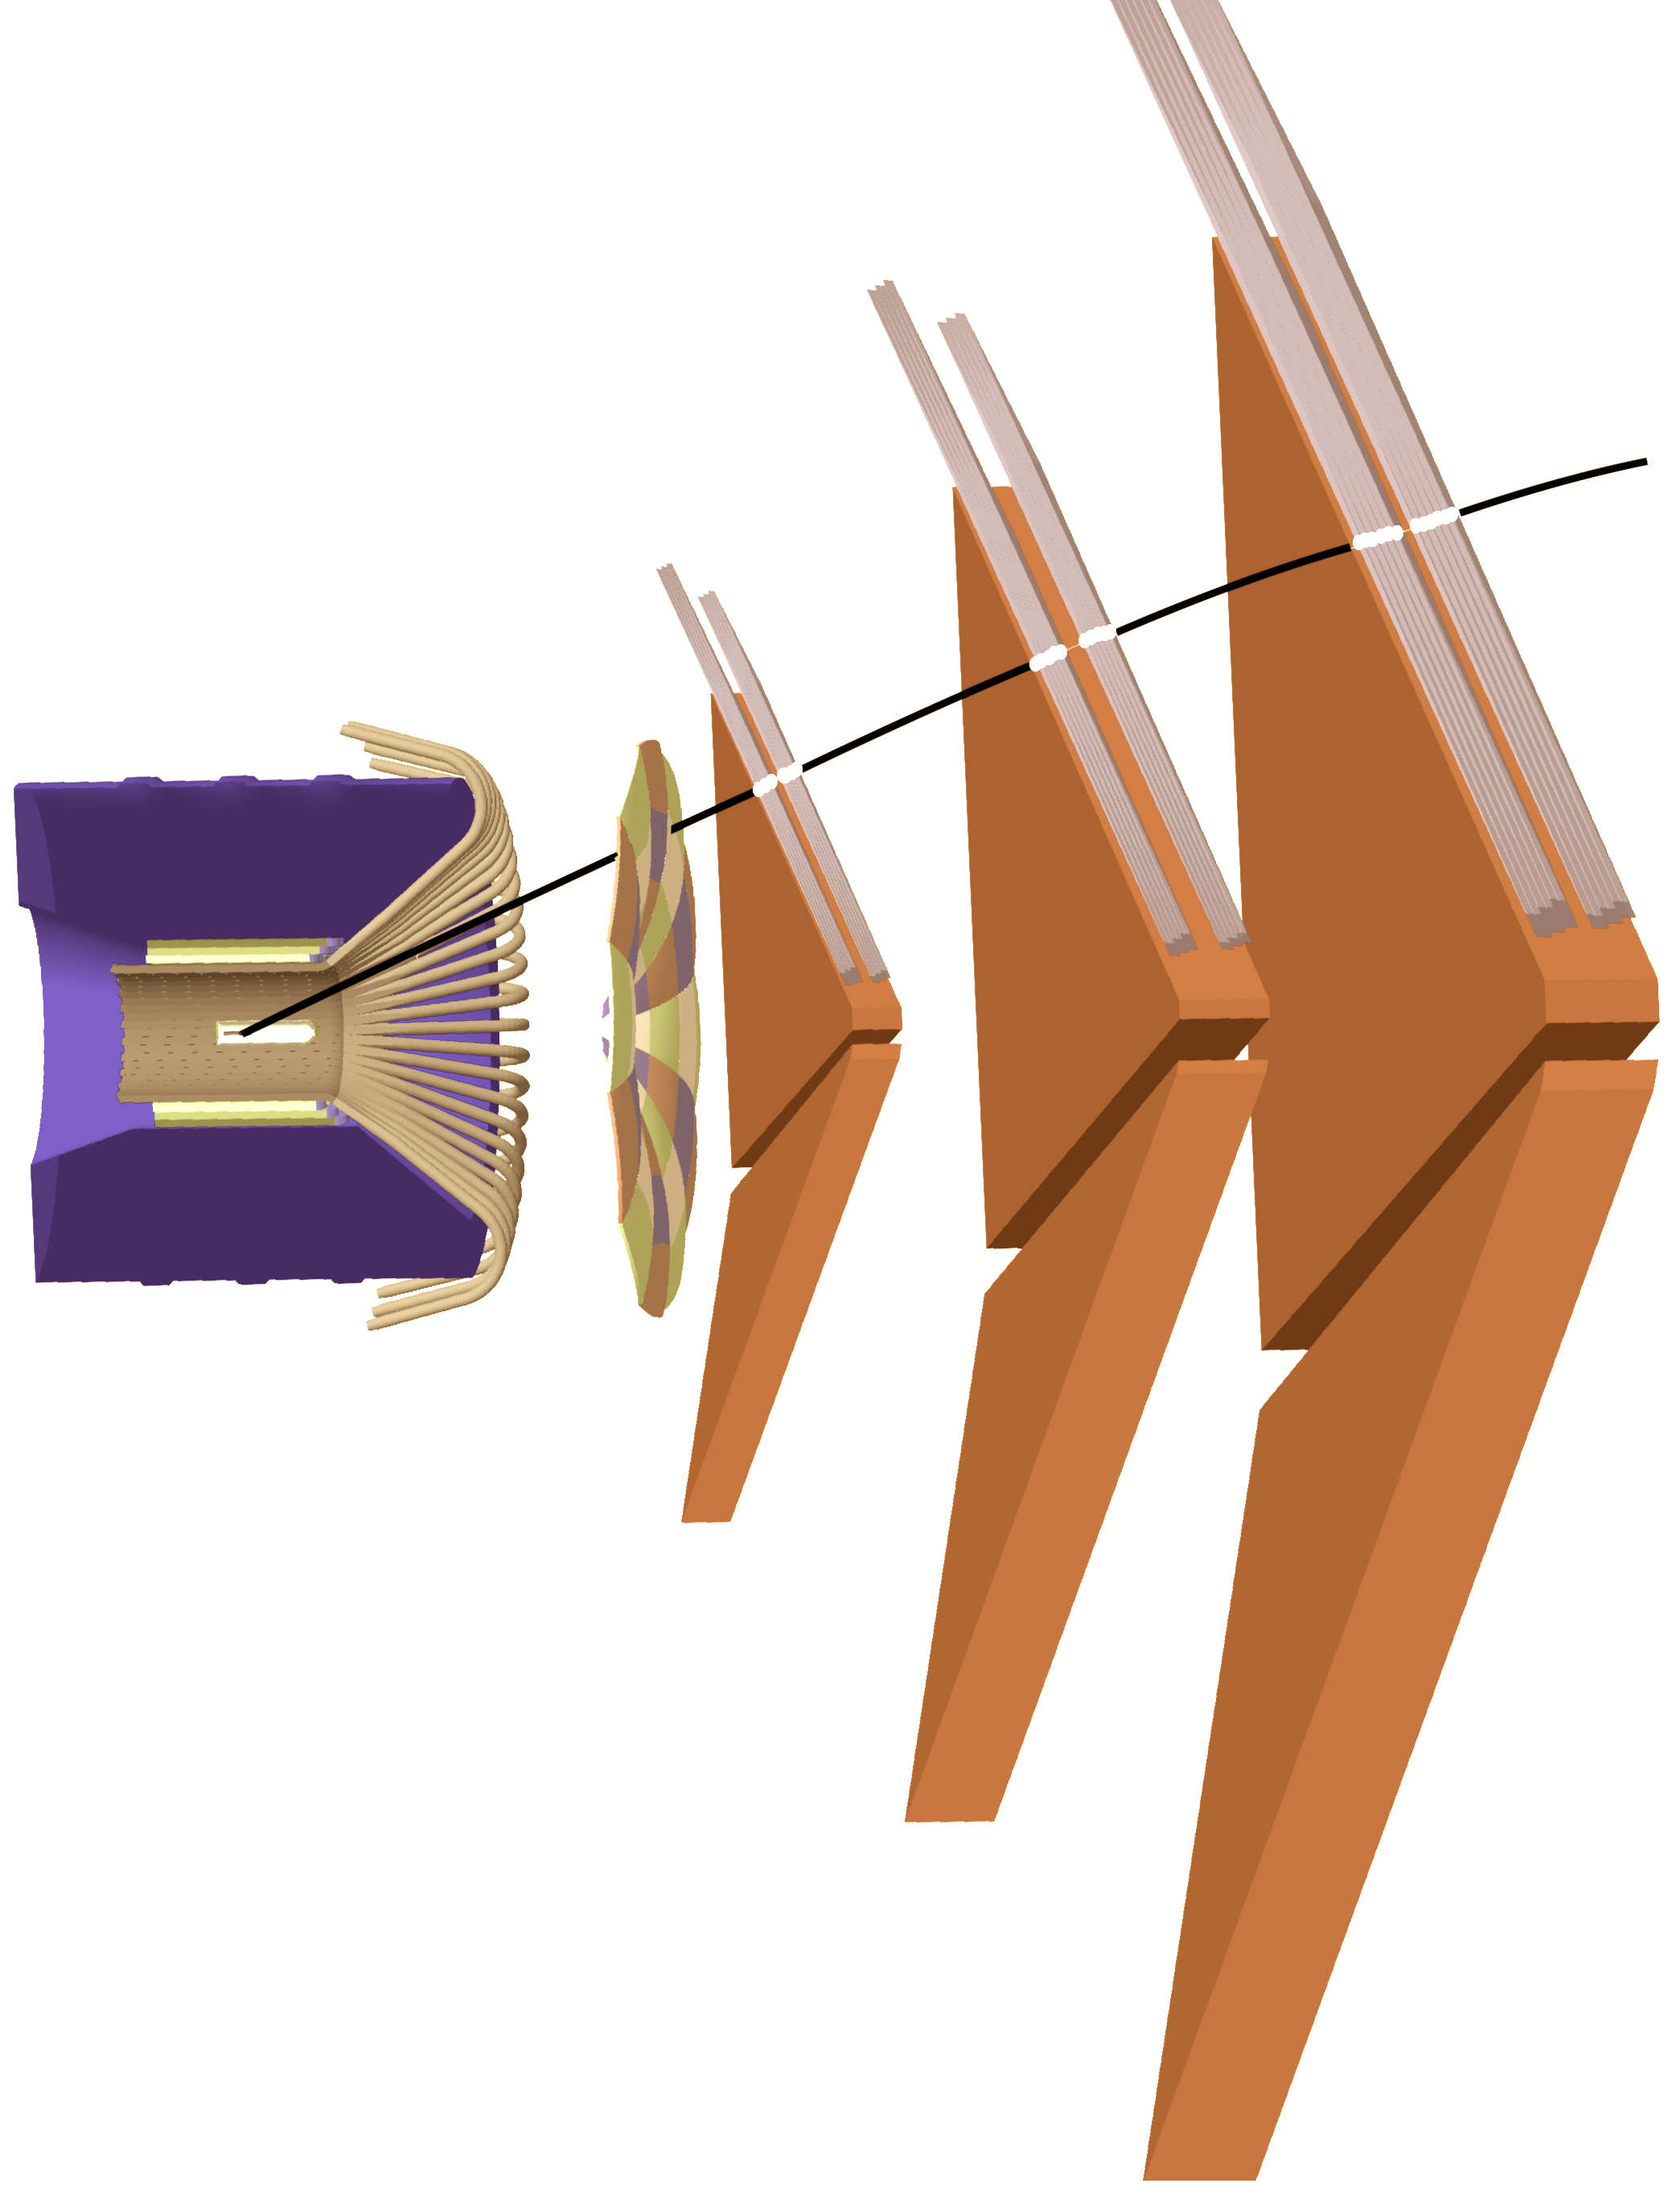
\includegraphics[width=0.95\columnwidth,keepaspectratio]{img/dcGeometry.png}
	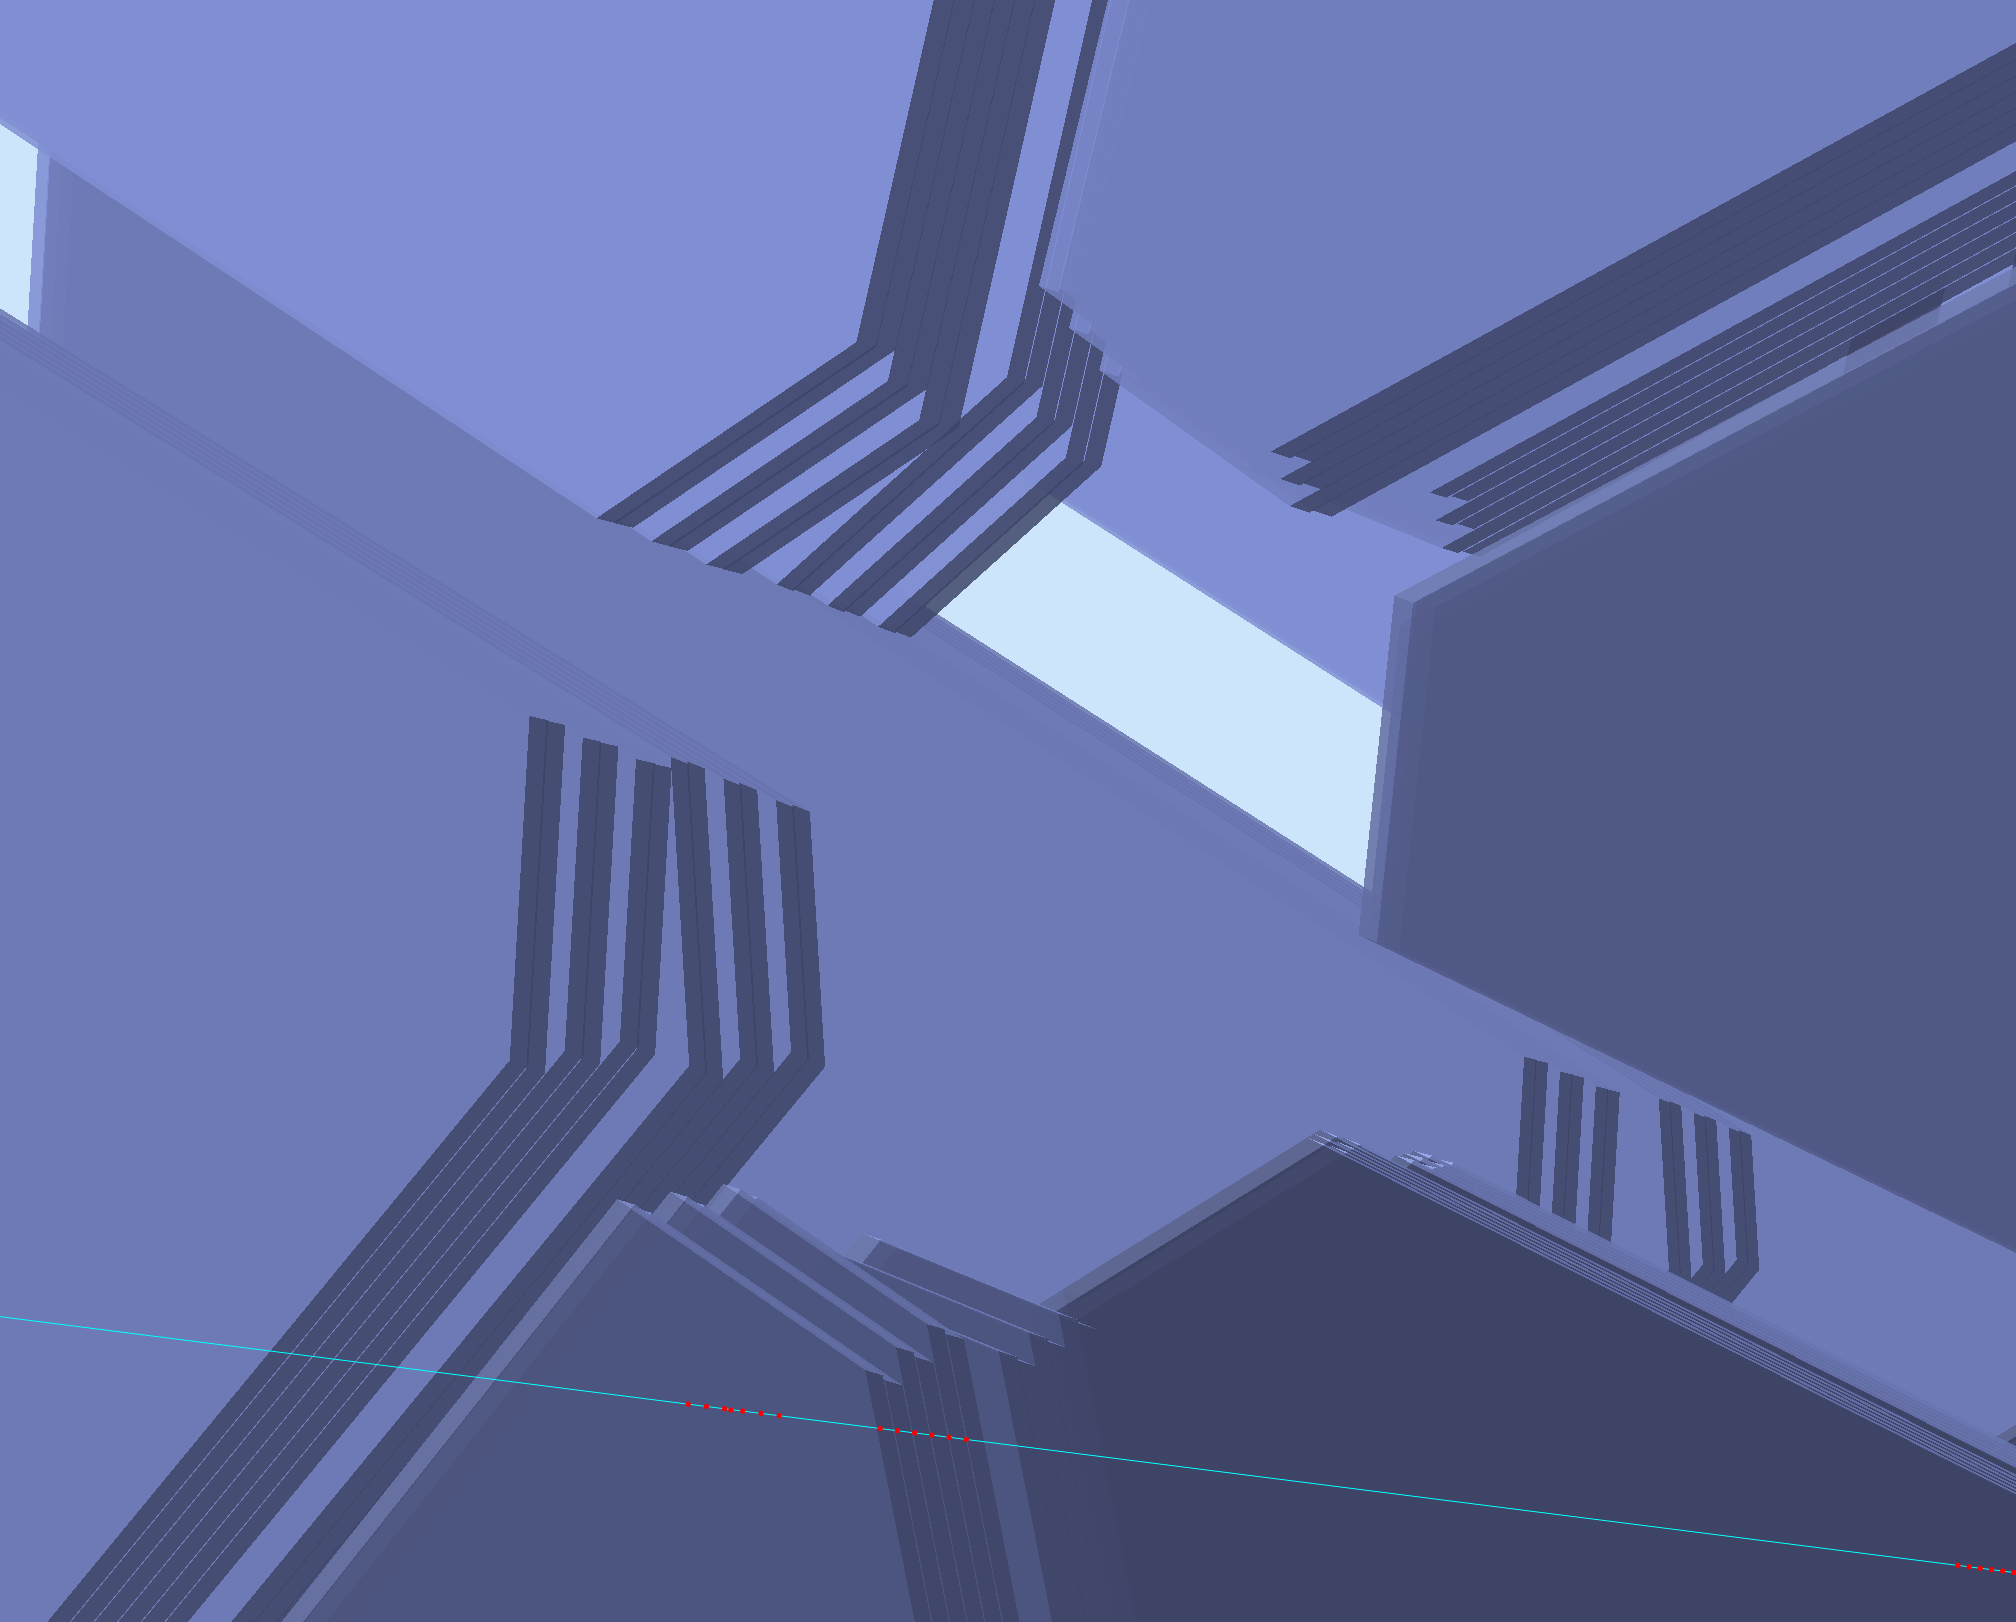
\includegraphics[width=0.95\columnwidth,keepaspectratio]{img/dcDetail.png}
	\caption{Top: the GEMC implementation of the DC geometry. The red trapezoids are the mother volumes corresponding to DC regions 1, 2 and 3. The cyan track is an electron, hitting the various
		      layers inside each region (a red dot / layer is a hit). Bottom: a zoom in near the beamline shows the Stereo angle layers. Six layers represent a DC superlayer.}
	\label{fig:dcGeometry}
\end{figure}


\subsubsection{Geometry Location on GitHub}
The Github location of the GEMC perl API script is \url{https://github.com/gemc/detectors/tree/master/clas12/dc}.
The geometry service definitions in coatjava is \url{https://github.com/JeffersonLab/clas12-offline-software/blob/development/common-tools/clas-jcsg/src/main/java/org/jlab/detector/geant4/v2/DCGeant4Factory.java}.

\subsection{Process ID}
At each Geant4 step, the local vertical position $y$ in the tilted g4Trap is computed. Knowing the distance
between each wire $\delta Y$ (given by the total height of the trapezoid divided by the number of wires, $112$), which is a constant as we're not taking into
account wire sagging, the wire ID is given by $n_i = y / \delta y$.

\subsection{Digitization}

\subsubsection{ADC}
There is no ADC calculation.

\subsubsection{TDC}
First, the distance of closest approach $DOCA$ is extrapolated for the hit. At each Geant4 step, the distance of the track from the wire is calculated.
The $DOCA$ is extracted among the points with energy deposited larger than $50 eV$, for which the sum of the step time + $DOCA / DV$ (where DV is the drift velocity) is minimal.

An initial time $T_i$ is calculated with a time to distance function which is the inverse of what extrapolated in calibration and used in reconstruction to go from TDC to $DOCA$.
The function takes into account:

\begin{itemize}
	\item the distance from the wire, in cm
	\item the cell size in superlayer
	\item the polar angle of the track
	\item magnitude of field in Tesla
\end{itemize}

A time walk correction function is applied to $T_i$ that includes discrete ionization effects based on the following input:

\begin{itemize}
	\item the distance from the wire, in cm
	\item the cell size in superlayer
	\item an adjustable factor (in mm) times $beta^2$ of the particle, the factor is adjusted according to data at small distances from the wire
	\item a parameter to adjust the matching between the two time walk distributions
	\item the velocity of the particle
\end{itemize}

The resulting $T_w$ is then used in a Landau-function to mimic the detector response function.

An intrinsic random time walk correction $\sigma_{TW}$ due to multiple scattering is calculated and the time is smeared with
a Gaussian function using $\sigma_{TW}$ as the resolution.
Finally, a random number is thrown (between 0 and 1) and if it's above the efficiency function, calculated based on $DOCA$, the hit is rejected.

\begin{figure}
	\centering
	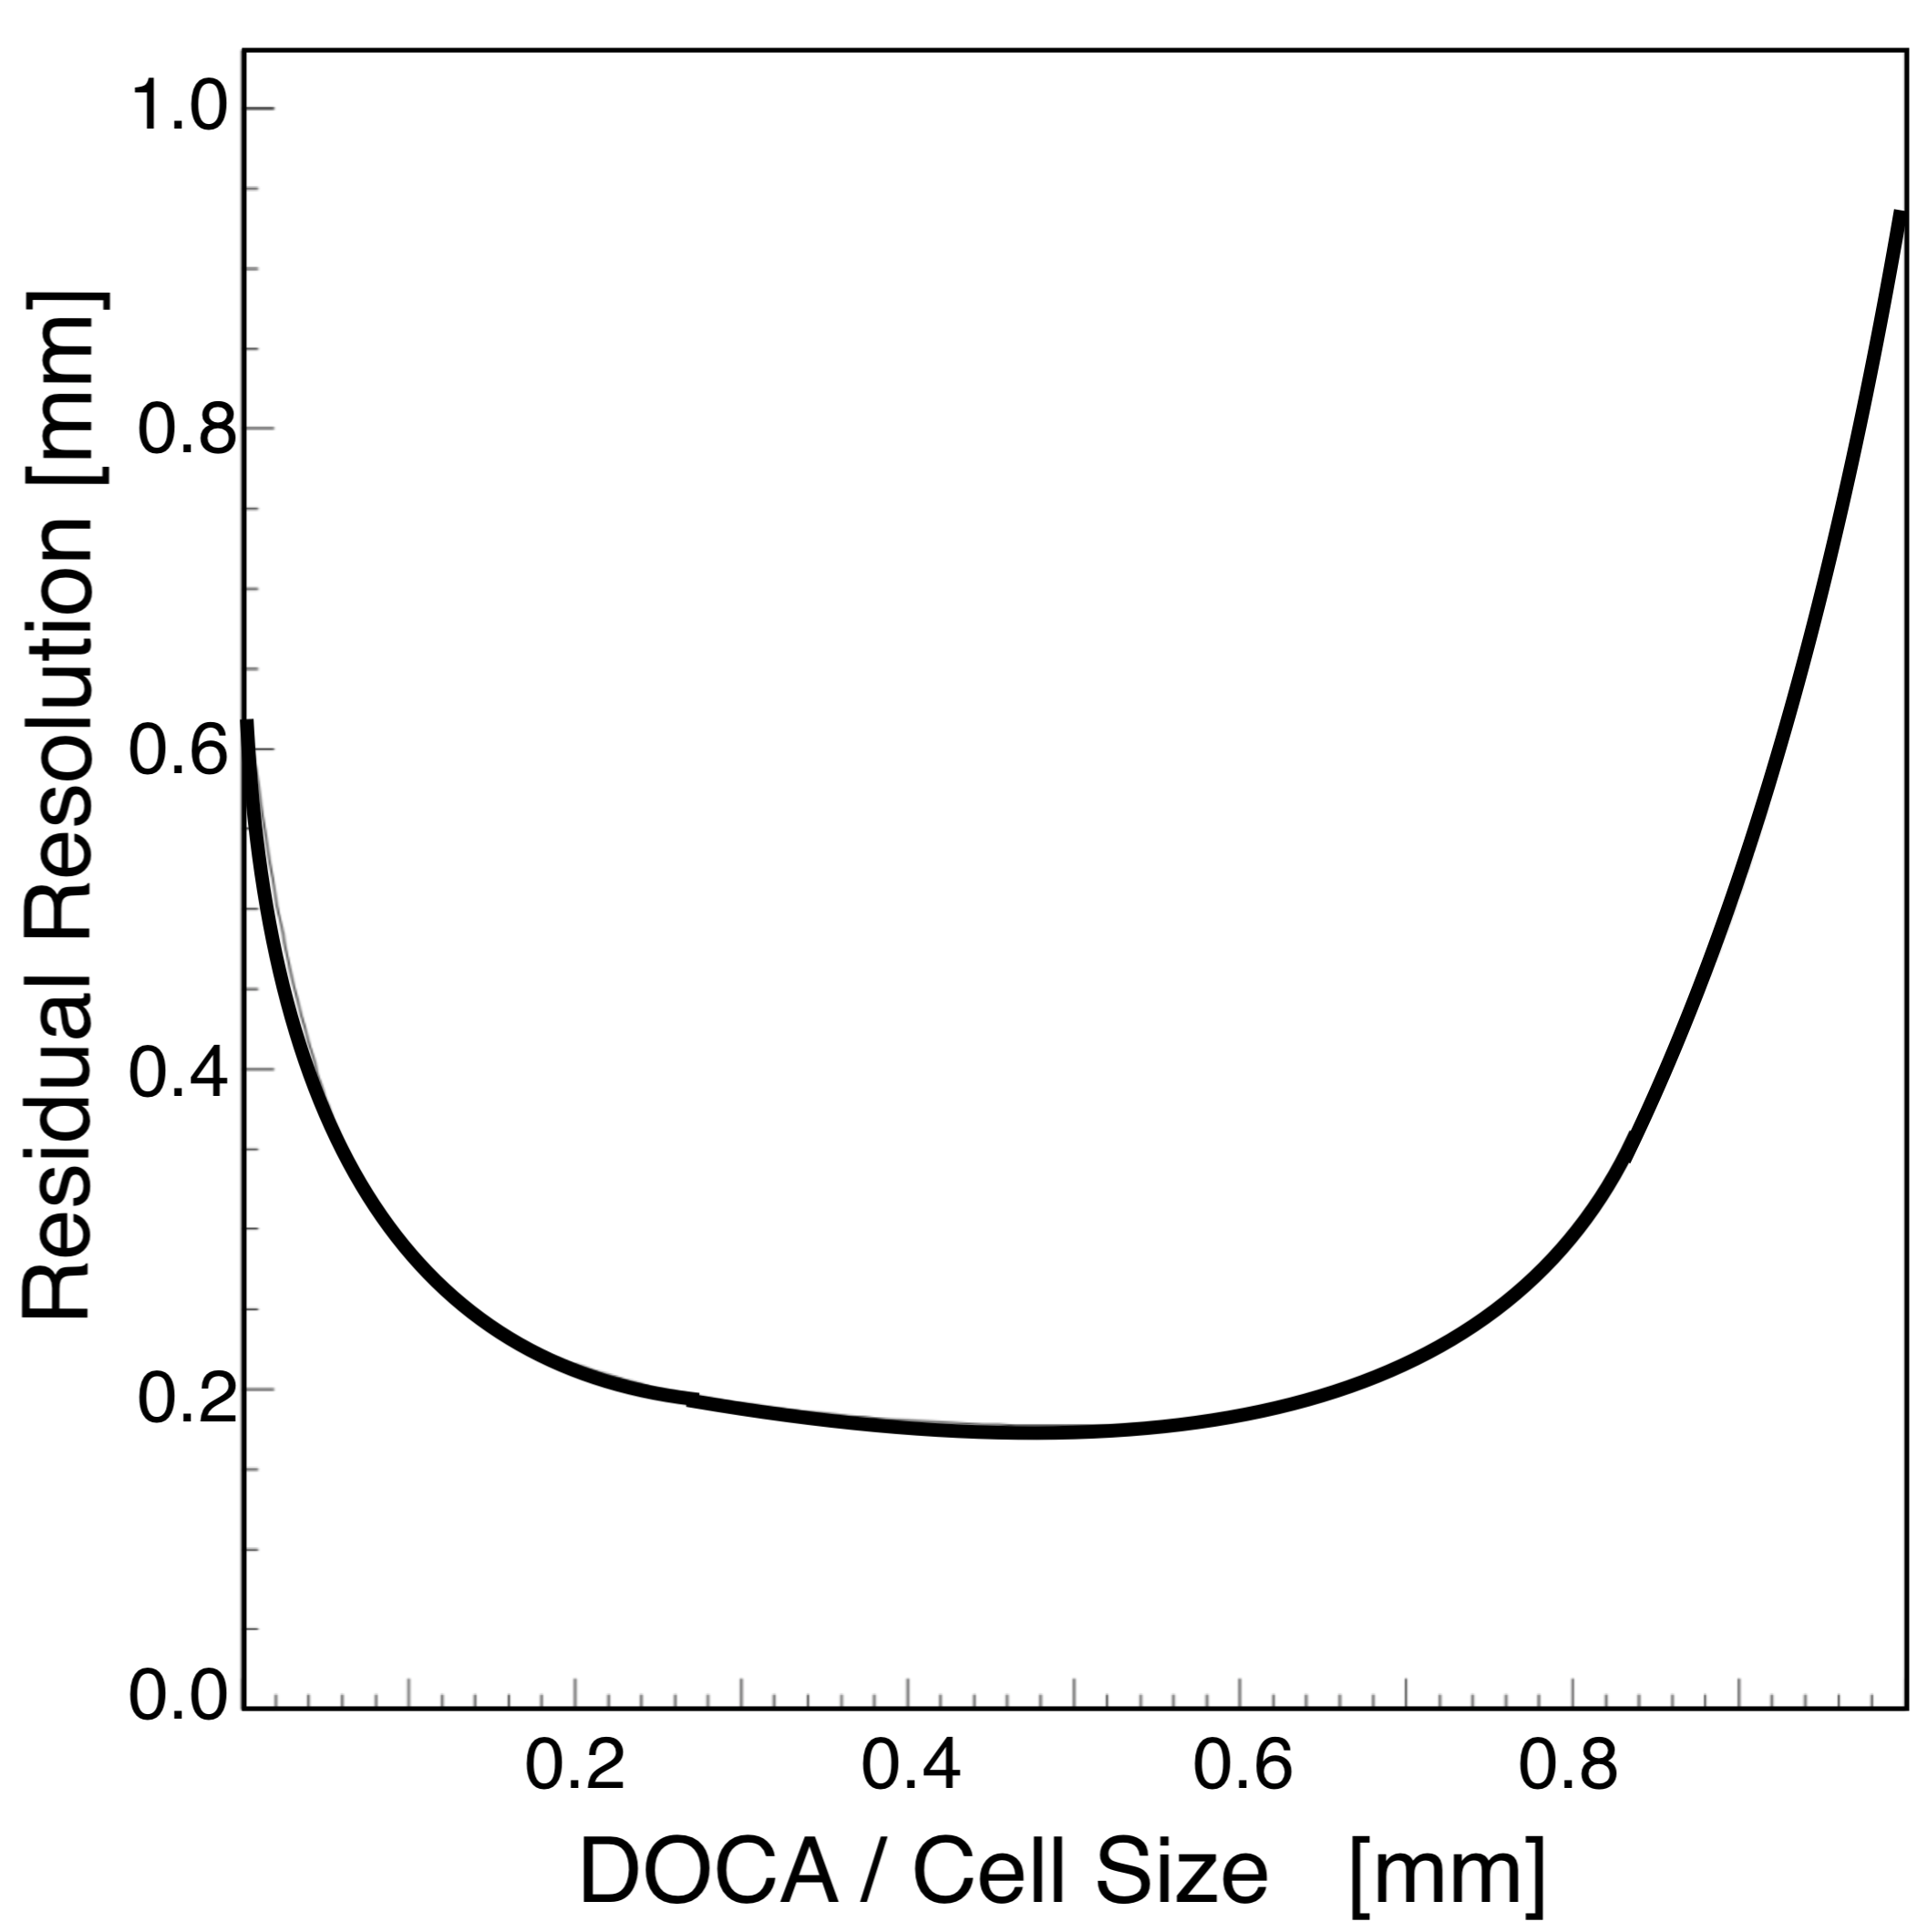
\includegraphics[width=0.95\columnwidth,keepaspectratio]{img/dcResolution.png}
	\caption{The fit to the data resolution provides parameters that are put in the CCDB database and read by the digitization routine at simulation run time.}
	\label{fig:dcResolution}
\end{figure}


\subsubsection{Summary of CCDB Table Used}
\begin{itemize}
	\item /calibration/dc/signal\_generation/intrinsic\_inefficiency
	\item /calibration/dc/signal\_generation/dc\_resolution
	\item /calibration/dc/time\_to\_distance/time2dist
	\item /geometry/dc/superlayer
\end{itemize}


\subsection{Digitized Bank}

The digitized output bank has $ID=1300$, and the variables are summarized in Table \ref{tab:dcBank}.

\begin{table}[h]
	\begin{center}
		\begin{tabular}{| c | c | c |}
			\hline \hline
			Variable         & Description  & Tag  \\
			\hline
               sector  &                                      sector index  &    1   \\
                layer  &                                       layer index  &    2   \\
                 wire  &                                        wire index  &    3   \\
                  tdc  &                                         tdc value  &    4   \\
                   LR  & Left/Right ambiguity                               &    5   \\
                 doca  & 2D distance of closest approach                    &    6   \\
                sdoca  &                                      smeared doca  &    7   \\
                 time  &              doca / drift velocity                 &    8   \\
                stime  &             sdoca / drift velocity                 &    9   \\
			\hline \hline
		\end{tabular}
	\end{center}
	\caption{The digitized DC bank.}\label{tab:dcBank}
\end{table}


\subsubsection{Time Window}

The time window  of the DC is set to 500 ns.

\subsubsection{Process Routine Git Repository Location}
The DC hit process routine location in git is \url{https://github.com/gemc/source/blob/master/hitprocess/clas12/dc_hitprocess.cc}


\subsubsection{Background Rates}

A detailed study of the background rates coming from beam interacting with the target was done to ensure that the DC occupancy stays
within limits that do not affect the reconstruction efficiency, typically below $5\%$.

Given the nominal operating luminosity $L=10^{35} cm^{-2}s^{-1}$, and the liquid hydrogen target of $5 cm$, the beam electron rates
is $R=4.7 \times 10^{11} Hz$. This corresponds to around 124,000 electrons in the DC 250 ns time window of region 1.

Various analyses \cite{targetStudy}, \cite{clas12Beamline}, \cite{clas12Background}, were performed using 124,000 electrons / event
to study the DC occupancy response to variations of hardware position and beamline configurations.
The results are summarized in \F{dcOccupancy}.

\begin{figure}
	\centering
	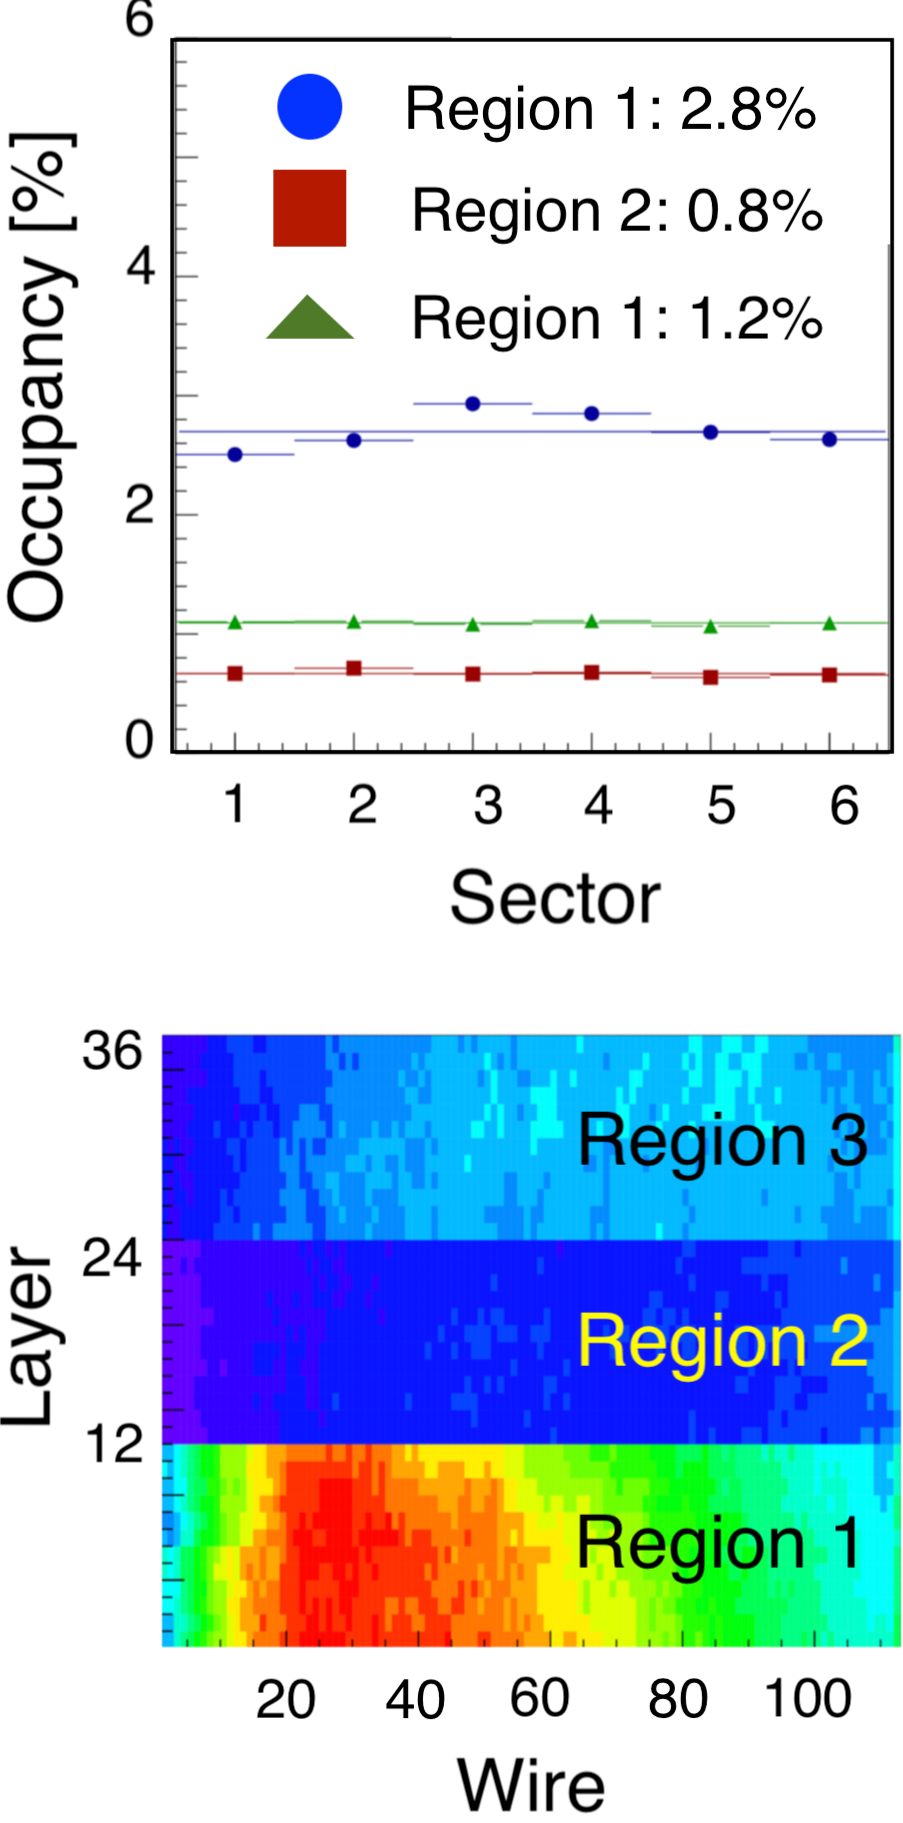
\includegraphics[width=0.95\columnwidth,keepaspectratio]{img/dcOccupancy.png}
	\caption{Results for DC rates for electron in-bending (left column) and out-bending (right column).
				Top: the occupancies are below $3\%$ for region 1 and below $1.2\%$ for region 3. Bottom: layer
				versus wire hit distribution: the two torus polarities show very similar distributions.}
	\label{fig:dcOccupancy}
\end{figure}

